\documentclass{article}
%
% Demo of the mcode package from 
% http://www.mathworks.co.uk/matlabcentral/fileexchange/8015-m-code-latex-package
% Updated 06 Mar 2014
%

\usepackage{graphicx}
\usepackage{wrapfig}
\usepackage{mathtools}
\usepackage{mathrsfs}
\usepackage{enumitem}
\usepackage{pdflscape}
\usepackage{color}
\usepackage{float}

\graphicspath{ {images/} }

% load package with ``framed'' and ``numbered'' option.
\usepackage[framed,numbered,autolinebreaks,useliterate]{mcode}

% something NOT relevant to the usage of the package.
\usepackage{url}
\setlength{\parindent}{0pt}
\setlength{\parskip}{18pt}


% //////////////////////////////////////////////////

\begin{document}

\title{Homework 5 - Optimal Control Systems}
\author{Erivelton Gualter dos Santos, 2703806}
\date{}

\maketitle 

\section{State the fundamental theorem of the calculus of variations}

According to Kirk in [1] the fundamental theorem of calculus of variations can be stated that the variation of a functional must be zero for an extremal. 

It means that for the following conditions:
\begin{enumerate}
\item Vector function of $t$ in the class $\Omega$;
\item $J(x)$ be a differentiable functional of $x$;
\item $\Omega$ includes functions that are not constrained by
any boundaries;
\item $x^*$ is an extremal (maximum or minimum);
\end{enumerate} 
Then,
\begin{equation}
\delta J(x^*,\delta x) = 0
\end{equation}
for all admissible $\delta x$. Where $\delta J$ is the variation of the functional $J$.


\section{Find the extremals}

\begin{enumerate}
\item[\textbf{a}] $ J(x) = \int_{a}^{b} 12xy + (y')^2 dx $  
\end{enumerate}

The solution of this problem can be found using the Euler Equation:
\begin{eqnarray}
\frac{\partial g}{\partial y} - \frac{d}{dt}\frac{\partial q}{\partial \dot{y}} = 0
\end{eqnarray}
Therefore, for $g(y,\dot{y}, x) = 12xy+y'^2 $, we have:
\begin{eqnarray*}
\begin{split}
\frac{\partial g}{\partial y} &= 12x \\
\frac{\partial q}{\partial \dot{y}} &= 2y'\\
\frac{d}{dt}\frac{\partial q}{\partial \dot{y}} &= 2y''
\end{split}
\end{eqnarray*}

Therefore:
\begin{eqnarray*}
\frac{\partial g}{\partial y} - \frac{d}{dt}\frac{\partial q}{\partial \dot{y}} = 12x - 2y'' = 0
\end{eqnarray*}
The second-order linear ordinary differential equation also can be written as : 
\begin{equation}
\frac{d^2y(x)}{dx^2} = 6x
\end{equation}
Integrate both side with respect to x:
\begin{eqnarray*}
\frac{dy(x)}{dx} = \int_{a}^{b} 6x \:\:dx = 3x^2 + C_1
\end{eqnarray*}
Integrate again both side with respect to x:
\begin{eqnarray*}
y(x) = \int_{a}^{b} 3x^2 + C_1 \:\:dx = x^3 + C_1x + C_2
\end{eqnarray*}

Therefore $y(x) = x^3 + C_1x + C_2 $ with initial and final conditions:
\begin{eqnarray*}
\begin{split}
y(a) &= y_a \\
y(b) &= y_b \\
\end{split}
\end{eqnarray*}

The constants $C 1$ and $C 2$ can be found by applying the boundary conditions.

\begin{enumerate}
\item[\textbf{b}] $ J(x) = \int_{a}^{b} y^2 + (y')^2 dx $  
\end{enumerate}

The solution of this problem can be found using the Euler Equation:
\begin{eqnarray}
\frac{\partial g}{\partial y} - \frac{d}{dt}\frac{\partial q}{\partial \dot{y}} = 0
\end{eqnarray}
Therefore, for $g(y,\dot{y}, x) = y^2 + (y')^2 $, we have:
\begin{eqnarray*}
\begin{split}
\frac{\partial g}{\partial y} &= 2y \\
\frac{\partial q}{\partial \dot{y}} &= 2y' \\
\frac{d}{dt}\frac{\partial q}{\partial \dot{y}} &= 2y''
\end{split}
\end{eqnarray*}

Therefore:
\begin{eqnarray*}
\frac{\partial g}{\partial y} - \frac{d}{dt}\frac{\partial q}{\partial \dot{y}} = 2y - 2y'' = 0
\end{eqnarray*}
The second-order linear ordinary differential equation also can be written as : 
\begin{equation}
\frac{d^2y(x)}{dx^2} - y = 0
\end{equation}

The solution for this second-order linear ordinary differential equation is:
\begin{eqnarray*}
y(x) = C_1 e^x + C_2 e^{-x}
\end{eqnarray*}
with initial and final conditions:
\begin{eqnarray*}
\begin{split}
y(a) &= y_a \\
y(b) &= y_b \\
\end{split}
\end{eqnarray*}

The constants $C_1$ and $C_2$ can be found by applying the boundary conditions.

\section{Verification of solution of Brachistochrone} 

\begin{eqnarray*}
\left \{
\begin{split}
x &= x_f +\frac{y_f}{2\cos^2\theta}_f [2(\theta_f-\theta) +\sin(2\theta_f)-\sin(2\theta)] \\
y &= \frac{y_f \cos^2\theta}{\cos^2\theta_f}
\end{split}
\right .
\end{eqnarray*}

The aim if verify if the following equation is true:
\begin{equation}
1+\dot{y}^2+2y\ddot{y} = 0
\end{equation}
To find $\dot{y}$ we can use the following expression:
\begin{eqnarray*}
\dot{y} = \frac{dy}{d\theta}\frac{d\theta}{dx}
\end{eqnarray*}
where:
\begin{eqnarray*}
\frac{d\theta}{dx} = {\left( \frac{d\theta}{dx} \right)}^{-1}
\end{eqnarray*}
\begin{eqnarray*}
\begin{split}
\frac{dy}{d\theta} &= -2y_f \frac{\cos\theta\sin\theta}{\cos^2\theta_f}\\
\frac{dx}{d\theta} &= -y_f\frac{1+\cos\left(2\theta\right)}{\cos^2\left(\theta_f\right)}\\
\end{split}
\end{eqnarray*}

Therefore:
\begin{eqnarray}
\dot{y} = 2\textcolor{blue}{y_f} \frac{\cos\theta\sin\theta}{\textcolor{red}{\cos^2\theta_f}}\frac{ \textcolor{red}{\cos^2\left(\theta_f\right)}}{\textcolor{blue}{y_f} \left[1+\cos\left(2\theta\right)\right]} = 2\frac{\cos\theta\sin\theta}{1+\cos\left(2\theta\right)}
\end{eqnarray}

According to Figure 1 and some mathematic derivation, we can write $ \cos\left(2\theta\right)$ equal to $2\cos^2\left(2\theta\right) -1$

Therefore:
\begin{eqnarray*}
\frac{d\dot{y}}{d\theta} = \frac{d}{d\theta}\left[2\frac{\cos\theta\sin\theta}{1+2\cos^2\left(2\theta\right) -1} \right] = \frac{\sin\theta}{\cos\theta}
\end{eqnarray*}

\begin{figure}[h]
\centering
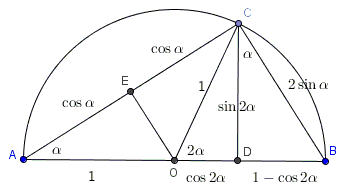
\includegraphics [width=3in]{DoubleAngle.png}
\caption{Illustration of trigonometric identities }
\end{figure} 

To find $\ddot{y}$ we can use the following expression:
\begin{eqnarray*}
\ddot{y} = \frac{d\dot{y}}{d\theta}\frac{d\theta}{dx}
\end{eqnarray*}
where:
\begin{eqnarray*}
\frac{d\dot{y}}{d\theta} = \frac{d}{d\theta}\left(\frac{\sin\theta}{\cos\theta}\right) = \frac{\cos^2\theta + \sin^2\theta}{\cos^2\theta}
\end{eqnarray*}



Therefore:
\begin{eqnarray*}
\begin{split}
\ddot{y} = \frac{d}{d\theta}\left(\frac{\sin\theta}{\cos\theta}\right) &= \left( \frac{\cos^2\theta + \sin^2\theta}{\cos^2\theta}\right)\left(- \frac{ \cos^2\left(\theta_f\right)}{y_f \left[1+\cos\left(2\theta\right)\right]} \right)\\
&= -\frac{\cos^2\theta + \sin^2\theta}{\cos^2\theta}\frac{ \cos^2\left(\theta_f\right)}{2y_f\cos^2\theta}
\end{split}
\end{eqnarray*}

Replacing the derived equations in: 
\begin{equation*}
1+\dot{y}^2+2y\ddot{y} = 0
\end{equation*}

\begin{eqnarray*}
\begin{split}
1 + \left( \frac{\sin\theta}{\cos\theta} \right)^2 + 2 \left(\frac{y_f \cos^2\theta}{\cos^2\theta_f} \right)\left( -\frac{\cos^2\theta + \sin^2\theta}{\cos^2\theta}\frac{ \cos^2\left(\theta_f\right)}{2y_f \cos^2\theta}\right) &= 0 \\ 
1 + \left( \frac{\sin\theta}{\cos\theta} \right)^2 + \textcolor{magenta}{2} \left(\frac{\textcolor{red}{y_f} \textcolor{blue}{\cos^2\theta}}{\textcolor{green}{\cos^2\theta_f}} \right)\left( -\frac{\cos^2\theta + \sin^2\theta}{\cos^2\theta}\frac{ \textcolor{green}{\cos^2\left(\theta_f\right)}}{\textcolor{magenta}{2}\textcolor{red}{y_f} \textcolor{blue}{\cos^2\theta}}\right) &= 0 \\ 
1 + \left( \frac{\sin\theta}{\cos\theta} \right)^2 - \frac{\cos^2\theta + \sin^2\theta}{\cos^2\theta} &= 0 \\ 
\end{split}
\end{eqnarray*}
Knowing that $ \cos^2\theta + \sin^2\theta = 1 $ and $ \cos^2\theta = \sin^2\theta -1 $, we have
\begin{eqnarray*}
\begin{split}
1 + \left( \frac{\sin\theta}{\cos\theta} \right)^2 - \frac{1}{\sin^2\theta -1 } &= 0 \\ 
\frac{\sin^2\theta\cos^2\theta \textcolor{red}{-\cos^2\theta} + \sin^4\theta -\sin^2\theta \textcolor{red}{+ \cos^2\theta}}{\cos^2\theta\left[\sin^2\theta-1 \right]} &= 0 \\ 
\frac{\sin^2\theta \left( \cos^2\theta + \sin^2\theta - 1 \right)}{\cos^2\theta\left[\sin^2\theta-1 \right]} &= 0 \\
1 - 1 &= 0
\end{split}
\end{eqnarray*}

 
\section{Plot the Brachistochrone Solution }

The figure 2-4 contains the brachistochrone solution for the desired final conditions: (1, 1), (1, 3), and (3, 1).

The figure 4 is an additional figure with the goal to verify the principle of optimality. This figure contains two solution: the first one is the final condition equal to (1,1) and the second one is a point in the optimal path from the previous solution. We can verify that the optimal path is the same for both. 

\begin{figure}[H]
\centering
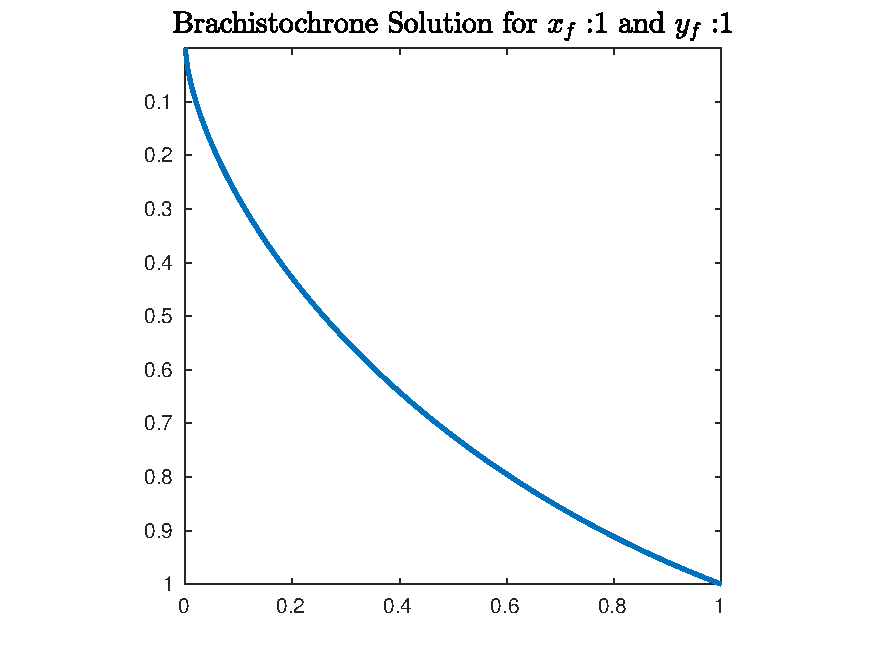
\includegraphics [width=4.4in]{f1}
\caption{brachistochrone solution for (1,1)}
\end{figure}
\begin{figure}[H]
\centering
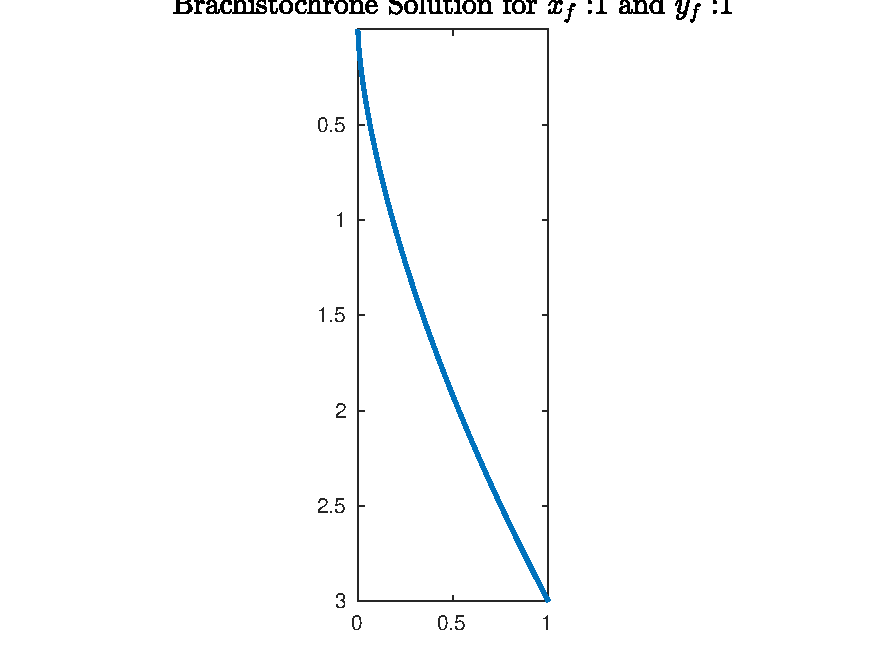
\includegraphics [width=4.4in]{f2}
\caption{brachistochrone solution for (1,3)}
\end{figure}

\begin{figure}[H]
\centering
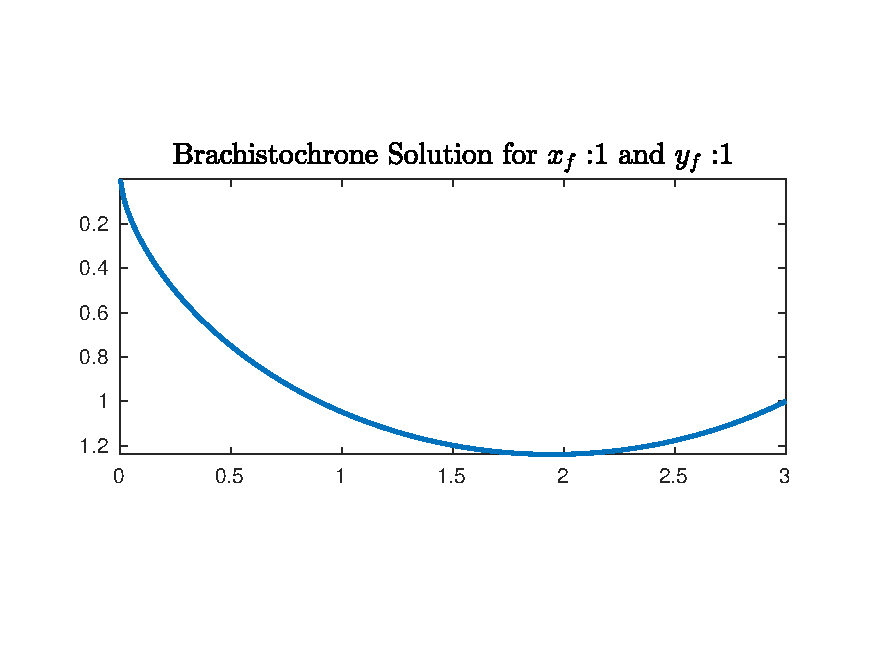
\includegraphics [width=4.4in]{f3}
\caption{brachistochrone solution for (3,1)}
\end{figure}
\begin{figure}[H]
\centering
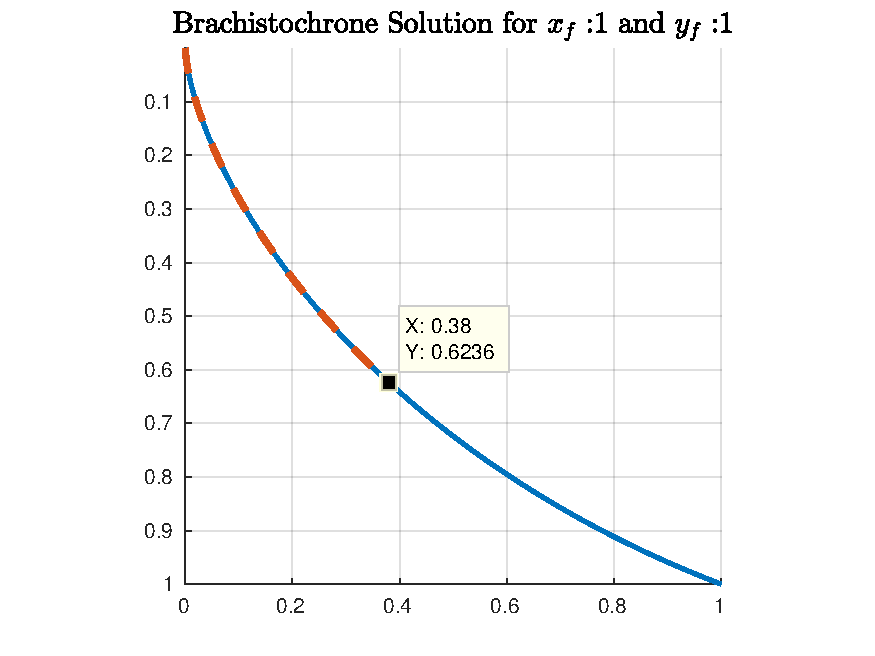
\includegraphics [width=4.4in]{f4}
\caption{brachistochrone solution to verify the principle of
optimality}
\end{figure}


\begin{lstlisting}
% Book: Optimal Control Theory: An introduxtion by Donald E. Kirk
%
% Erivelton Gualter, 02/21/2018

clear all; clc; close all

% parameter
theta0 = pi/2;
X0 = 0; 
Y0 = 0;
    
Xf = [1, 1, 3]; 
Yf = [1, 3, 1];

[X(1,:), Y(1,:)] = brachistochrone(X0, Y0, Xf(1), Yf(1), theta0);
[X(2,:), Y(2,:)] = brachistochrone(X0, Y0, Xf(2), Yf(2), theta0);
[X(3,:), Y(3,:)] = brachistochrone(X0, Y0, Xf(3), Yf(3), theta0);

Xf(4) = 0.380000000000000; 
Yf(4) = 0.623586752778062;
[X(4,:), Y(4,:)] = brachistochrone(X0, Y0, Xf(4), Yf(4), theta0);
    
f1 = figure; plot(X(1,:),Y(1,:), 'LineWidth', 2); 
set(gca, 'Ydir','reverse');
title_str = strcat('Brachistochrone Solution for $x_f: $',num2str(Xf(1)),' and $y_f: $',num2str(Yf(1)));
title(title_str, 'Interpreter','Latex', 'FontSize',14);
axis equal; axis([min(X(1,:)) max(X(1,:)) min(Y(1,:)) max(Y(1,:))]);
saveFigureToPdf('f1',f1);

f2 = figure; plot(X(2,:),Y(2,:), 'LineWidth', 2); 
set(gca, 'Ydir','reverse');
title_str = strcat('Brachistochrone Solution for $x_f: $',num2str(Xf(1)),' and $y_f: $',num2str(Yf(1)));
title(title_str, 'Interpreter','Latex', 'FontSize',14);
axis equal; axis([min(X(2,:)) max(X(2,:)) min(Y(2,:)) max(Y(2,:))]);
saveFigureToPdf('f2',f2);

f3 = figure; plot(X(3,:),Y(3,:), 'LineWidth', 2); 
set(gca, 'Ydir','reverse');
title_str = strcat('Brachistochrone Solution for $x_f: $',num2str(Xf(1)),' and $y_f: $',num2str(Yf(1)));
title(title_str, 'Interpreter','Latex', 'FontSize',14);
axis equal; axis([min(X(3,:)) max(X(3,:)) min(Y(3,:)) max(Y(3,:))]);
saveFigureToPdf('f3',f3);

f4 = figure; hold on; 
plot(X(1,:),Y(1,:), 'LineWidth', 2); plot(X(4,:),Y(4,:), '--', 'LineWidth', 3); 
set(gca, 'Ydir','reverse');
title_str = strcat('Brachistochrone Solution for $x_f: $',num2str(Xf(1)),' and $y_f: $',num2str(Yf(1)));
title(title_str, 'Interpreter','Latex', 'FontSize',14);
axis equal; axis([min(X(1,:)) max(X(1,:)) min(Y(1,:)) max(Y(1,:))]);
legend('[0,0]-[1,1]','[0,0]-[0.4,0.6]');
saveFigureToPdf('f4',f4);

function [X,Y] = brachistochrone(X0, Y0, xf, yf, theta0)

    N = 200;

    fun = @(thetaf) f1([X0; Y0], [xf; yf], theta0, thetaf);  % function of x alone
    tf = fzero(fun,0);

    X = X0:(xf-X0)/N:xf(1);
    for i=1:length(X)

        fun = @(theta) f2(X(i), [xf; yf], theta, tf);  % function of x alone
        theta_out = fzero(fun,0);

        Y(i) = yf*cos(theta_out)^2/(cos(tf)^2);

    end
    
    % Functions
    function minxy = f1(P0, Pf, theta, thetaf)

        x = P0(1);
        y = P0(2);
        xf = Pf(1);
        yf = Pf(2);

        minxy = x - (xf + yf/(2*cos(thetaf)^2) * (2*(thetaf-theta) + ...
            sin(2*thetaf)) - sin(2*theta));

        minxy = minxy + y - yf/(2*cos(thetaf)^2)*cos(theta)^2;
    end

    function minx = f2(x, Pf, theta, thetaf)

        xf = Pf(1);
        yf = Pf(2);

        minx = x - (xf + yf/(2*cos(thetaf)^2) * (2*(thetaf-theta) + sin(2*thetaf) ...
            - sin(2*theta)));
    end
end
\end{lstlisting}

You can access the code at: https://github.com/EriveltonGualter/EEC-744-Optimal-Control-Systems

\end{document}
